\section{Implementation} \label{sec:implementation}
The implementation is based on a Kubernetes master in the cloud and and one worker on-premises. The master runs on a virtual private server (VPS) from Contabo\cite{online:ContaboWebsite}. 
It has four cores, a minimum of 10 gigabyte of RAM and runs Ubuntu 18.10, which is more then the official Kubernetes requirments\cite{kubernetesRequirementsInstall:online}. 
In an interview with Oracle Cloud Platform Architect Allan H{\o}jgaard Jensen he said "only bare metal offers the best speeds". However, getting a full server was not possible and would have not changed much, as performance on the master is not an issue. The worker is a raspberry pi model 3b+ on bare metal as here performance is critical. 
It only has one gigabyte of RAM and runs on ARMv7, based on a 32-bit architecture. Even though it meets the Kubernetes system requirements for workers it is generally not recommended by the Kubernetes developers. But, as the Raspberry Pi 3b+ is one of the most popular single-board computers and often used in IoT project, I use it in this thesis as well. \Cref{fig:baSetup} shows the architectural setup of this thesis.
\begin{figure}[h!]
    \centering
    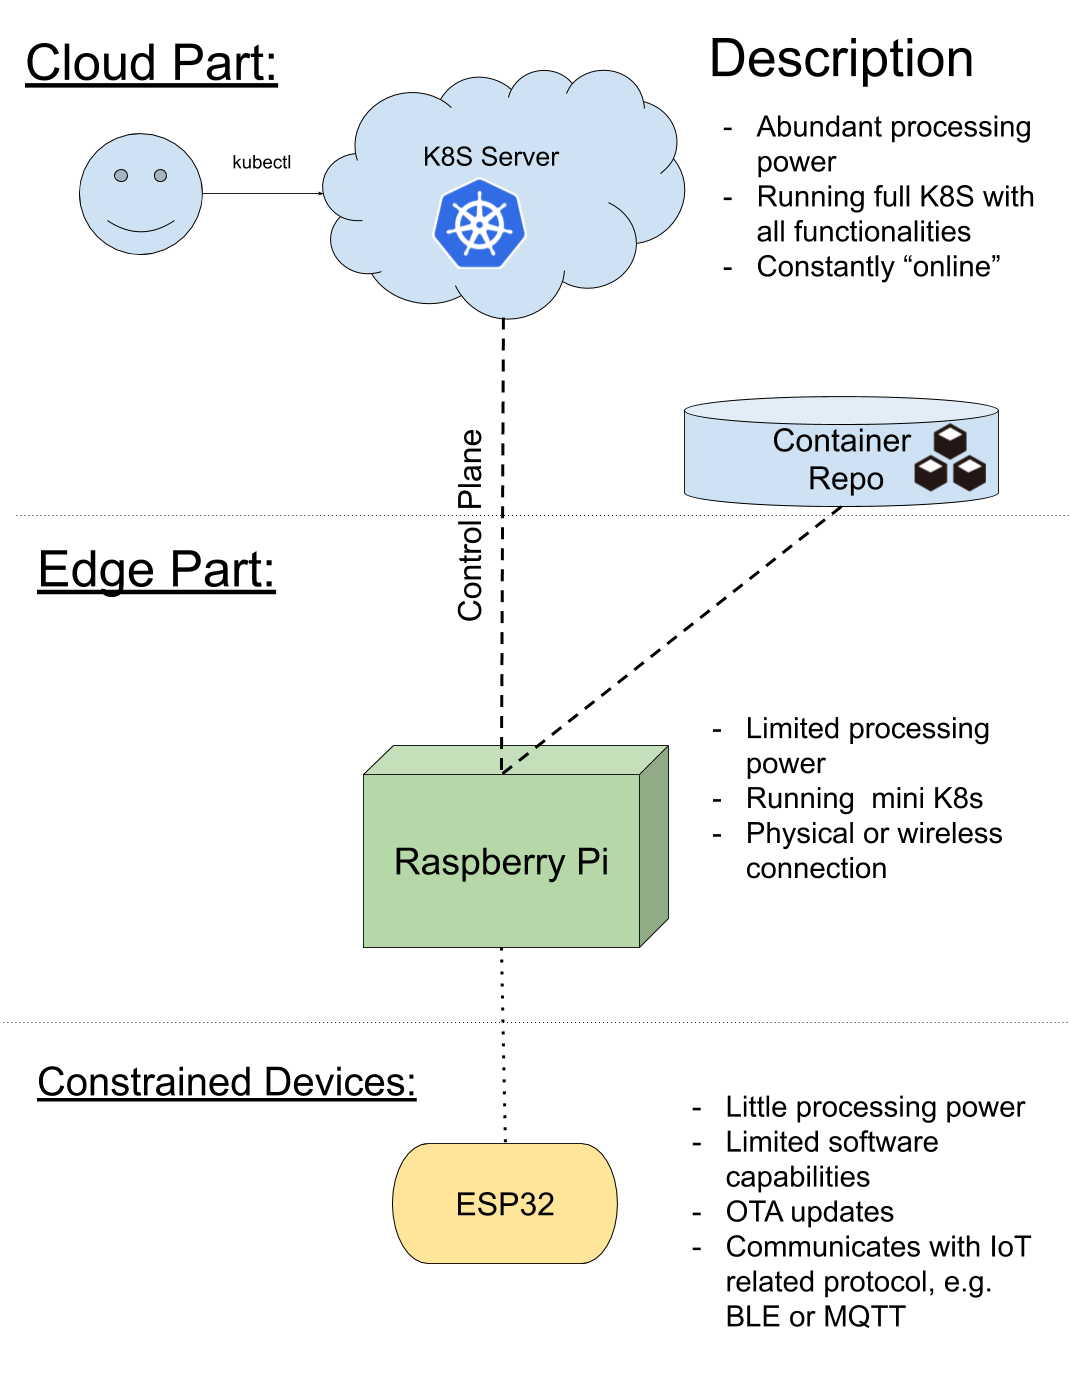
\includegraphics[scale=0.15]{figures/baSetup.png}
    \caption{Thesis implementation setup.}
    \label{fig:baSetup}
\end{figure}
I will divide the implementation in different stages to describe better what challenges arise from using Kubernetes on the edge as IoT Gateway. In stage one I just setup the system, installing the edge device and joining it to the master. In stage two, I will deploy a example application to the edge device controlled from the Kubernetes master and I will explain in more detail the build steps for the containers. In stage three the IoT components will be deployed. This includes a MQTT server inside Kubernetes and a microcontroller subscribing and publishing to that server. The master should also be able to initiate updates to IoT devices which support OTA updates from the Raspberry Pi. In stage 4 further features will be implemented. Finally, in stage 5 I will come back and revisit and try to implement issues I found in the stages before.\\


\subsection{Kubernetes Installation}
The Kubernetes master installation is well documented and did not pose any troubles. For completion of this thesis I will briefly mention the additional components installed on the master. Kubernetes has no default networking implementation, thus I installed Flannel\cite{coreosFlannel:online}, one of the simplest and most widely used networking fabrics specifically designed for Kubernetes. It runs a small binary called \textit{flanneld} on each node and provides networking between nodes and pods\footnote{The specifics of Flannels networking are outside this thesis scope, for more information see \url{https://blog.laputa.io/kubernetes-flannel-networking-6a1cb1f8ec7c}}. For administrative purposes I also installed the Kubernetes Dashboard.

The Raspberry Pi Foundation recently released an update to Raspbian (the RPi OS) called buster, which does dropped support of the aufs-dkms kernel modules, which are dependencies of kubeadm and containerd. The online community advised in forums to avoid the dependency but if possible switch back to the older version of Raspbian called stretch. Out of time concerns, I switched back to the old version. 

I switched the official Kubernetes kubelet with the kubelet binary from Ranchers K3s called Hyperkube. \Cref{fig:kubeBinaries} shows the size of the binary files of three most important components of Kubernetes, kubeadm, kubelet and kubectl.
\begin{figure}[h!]
    \centering
    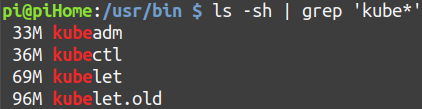
\includegraphics[scale=0.5]{figures/kubeBinariesSize.png}
    \vspace*{-0.3cm}
    \mycaption[The Sizes of the Kubernetes Binaries.]{\\ Note, \textit{kubelet} is the K3s hyperkube binary and \textit{kubelet.old} is the official kubelet bianry.}
    \label{fig:kubeBinaries}
\end{figure}
In total the official binaries are 165 megabyte large and the kubelet (\textit{kubelet.old} file) takes almost half the space. Using the K3s build of kubelet (\textit{kubelet} file) brings the total amount to 138 megabyte saving almost 20\% of space in addition to its other benefits discussed in \cref{sec:Kubernetes} \nameref{sec:Kubernetes}. The full installation procedure can be found in the repository of this thesis for replication and validation.

Finally, the effects on the system resources are two folds, the native applications and the running containers. The Raspberry Pi has 926MB total memory and a 1.4 GHz quad-core CPU. Firstly, \cref{fig:kubernetesResourceConsumption} shows the resource usage of the native applications
\begin{figure}[h!]
    \centering
    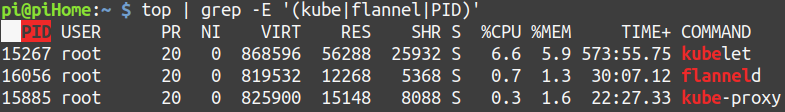
\includegraphics[scale=0.5]{figures/kubernetesResourceConsumption.png}
    \vspace*{-0.3cm}
    \caption[The Resource Usage of native Kubernetes Components.]{Using the K3s hyperkube binary.}
    \label{fig:kubernetesResourceConsumption}
\end{figure}
The kubelet process uses 6.6\% of the CPU and 5.9\% of the memory. While the memory usage is consistent, the CPU usage varies a lot and can reach peaks of 16\%. Using the command
\begin{displayquote}
\textit{top | egrep --line-buffered '(kubelet|PID)' > /home/pi/kubeletHyper.txt }
\end{displayquote}
the cpu usage was tracked over 38 minutes with an average of 3.16 data points per second and a total of 7235 data points\footnote{The entire statistics can be found in the project files together with the source code.}. The average CPU usage in the time period was 10.3\%, the memory usage was constant.

Flanneld and kube-proxy both use less than 1\% CPU and 1.3\% and 1.6\% of memory, respectively. It is important to note that the container runtime is not included in that statistics. The resource usage of the Kubernetes relevant containers is shown in \cref{fig:kubernetesResourceConsumptionCut}\footnote{The figure is cut to fit the page. The full figure can be seen the appendix.}.
\begin{figure}[h!]
    \centering
    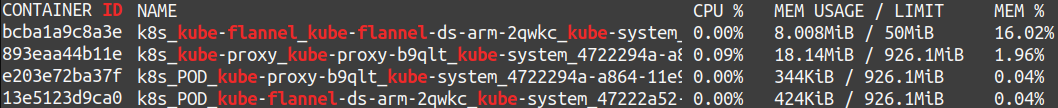
\includegraphics[scale=1.6]{figures/kubeContainerResourceUsageCut.png}
    \vspace*{-0.3cm}
    \caption[The Resource Usage of Kubernetes Containers.]{\\The command used is: \textit{docker stats | grep -E '(ID|kube|flannel)'}.}
    \label{fig:kubernetesResourceConsumptionCut}
\end{figure}
Flannel and kube-proxy consume 0.86\% and 1.96\% of the memory, respectively\footnote{flannel's limit is 50MB, hence the 16.02\% in the figure.}. The CPU usage of all containers is negligible at below 1\%. Adding up the numbers, after the installation Kubernetes uses 11.4\% of the CPU and 11.7\% of the total memory. This translates to 0.46GHz CPU usage, see \cref{eq:cpuTotal}, and 108.35MB memory usage, see \cref{eq:ramTotal}.
\begin{equation} \label{eq:cpuTotal}
    1.4GHz * 4 \; \textrm{(cores)} * 0.114 = 0.638GHz  \quad \textrm{(CPU usage)}
  \end{equation}
  \begin{equation} \label{eq:ramTotal}
    926.1MB * 0.117 = 108.354MB  \quad \textrm{(RAM usage)}
  \end{equation}
The memory consumption is especially concerning as swap needs to be disabled for Kubernetes to install. Swap is a partion in Linux used for paging. If disabled, memory can not be written to disk anymore which can lead to a memory overflow.
\subsection{Implementing a test Service} \label{sec:testService}
To test the Kubernetes setup I developed a simple go microservice called \textit{hello}. It listens on port 3000 and has three endpoints \textit{/hello/}, \textit{/hello/info} and \textit{/hello/path}. They don't implement any deeper logic but pose as an exemplary implementation for future services. I show exemplary Kubernetes configuration files and use this section to explain their meaning in more detail. For easier testability with cURL this microservice is based on json and not on protobufs.\\
\Cref{lst:dockerfileHello} shows the Dockerfile for building the microservice.
\lstset{
numbers=left, 
basicstyle=\footnotesize,
frame = single, 
language=Pascal, 
framexleftmargin=16pt,
% captionpos=b,
xleftmargin=2.3cm,
}
\begin{lstlisting}[linewidth=13cm, caption={Dockerfile for the Hello Application},label={lst:dockerfileHello}]
FROM golang:alpine as builder
EXPOSE 3000
COPY src .
RUN adduser -D -H -u 10001 scratchuser && \
    cd /go/main && \
    CGO_ENABLED=0 GOOS=linux GOARCH=arm GOARM=7 
    go build -a -installsuffix cgo -ldflags 
    '-extldflags "-static"' -o main .

FROM scratch
COPY --from=builder /etc/ssl/certs/ /etc/ssl/certs
COPY --from=builder /go/main/main /
COPY --from=builder /etc/passwd /etc/passwd
USER scratchuser
CMD ["./main"]
\end{lstlisting}
The code is cross-compiled in a builder container, which provides an isolated and replaceable build environment, this happens in line 1--8. Line 1 takes a fresh go alpine container with the latest go version. I then expose the port 3000 for the application to interact with its environment and copy the source code in the new container, line 2 and 3, respectively. Each new command produces a new temporary cached container, thus I the lines, 4--8, are all one \textit{RUN} command. It first adds a new user called \textit{scratchuser} without root privileges and the goes into the go main file directory and cross-compiles the application for ARMv7 (the last step is line 6--8). In lines 10--15, the final image is build. Line 10 initializes a new scratch container. This image is empty and thus uses a less memory and system resources. In lines 11--13 the relevant documents are copied in the new container. This includes the certificates from certificate authorities\footnote{They are important for encrypted connections.} (11), the application binary (12) and the user password (13). Line 14 switches to the scratchuser. This user has no root privileges and thus can never gain system control. Lastly, I specify the command run when a container based on the build image is run (15).\\
To see how important it is to use a scratch image as a base for memory purposes, consider \cref{fig:imageSizeComparison}. It shows just how much can be saved using this technique.
\begin{figure}[h!]
    \centering
    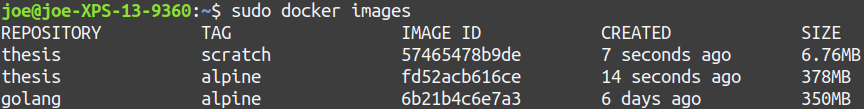
\includegraphics[scale=0.4]{figures/imageSizeComparison.png}
    \caption{The image sizes of the application.}
    \label{fig:imageSizeComparison}
\end{figure}
The go alpine image at the bottom is 350MB, the final image is a hefty 28MB bigger at 378MB (lines 1--8 in \cref{lst:dockerfileHello}). Copying the binary, the user files and the  certificates into a scratch image takes up only 6.76MB in total (lines 11--13). That is significantly smaller and with less overhead. When the container runs, only the binary is loaded and nothing else is running in the background. Contrast that to the alpine image where every time it is run, it starts a shell command line and includes an entire go build environment. The image is then tagged with a repository and tag name and pushed to the corresponding repository.\\
On the Kubernetes master I defined a service for the \textit{hello} application with the manifest shown in \cref{lst:serviceManifest}. It is an abstraction defining the guidelines how to access the pods inside a service, as the pods themselves are volatile\footnote{Each pod has a unique IP but Kubernetes does not guarantee for Pods and can reschedule pods at any moment}. It thus enables decoupling of the networking and the actual application from an outsiders perspective.
\lstset{
numbers=left, 
basicstyle=\footnotesize,
frame = single, 
language=Pascal, 
framexleftmargin=16pt,
% captionpos=b,
xleftmargin=2.3cm,
}
\begin{lstlisting}[linewidth=13cm, caption={The manifest of the \textit{hello} service.},label={lst:serviceManifest}]
apiVersion: v1
kind: Service
metadata:
  name: hello-service
  namespace: hello-namespace
spec:
  type: NodePort
  selector:
    app: hello
  ports:
    - name: http
      nodePort: 30001
      port: 3000
      targetPort: 3000
\end{lstlisting}
Line 5 tells the master that the service should be deployed in the namespace \textit{hello-namespace}. Line 6 specifies that each pod of this service should be accessible on the node it is scheduled on without going through the Kubernetes ingress resource. This is called nodeport and specified in line 12 to be \textit{30001}. Line 7 tells Kubernetes that the application corresponding to the service is called \textit{hello}. Finally, line 13 and 14 specify the ports the actual container expose.\\
For the actual state description of the application I use a \textit{Deployment} shown in \cref{lst:deploymentManifest}. A deployment specifies the desired state and the Deployment controller changes the actual state inside the cluster towards the desired state. 

\lstset{
numbers=left, 
basicstyle=\footnotesize,
frame = single, 
language=Pascal, 
framexleftmargin=16pt,
escapeinside=||,
xleftmargin=2.3cm,
}
\begin{lstlisting}[linewidth=13cm, caption={The Deployment Manifest of the \textit{hello} Application.},label={lst:deploymentManifest}]
apiVersion: apps/v1
kind: Deployment
metadata:
  name: hello-deployment
  namespace: hello-namespace |\Suppressnumber|
... |\Reactivatenumber{16}|
    spec:
      affinity:
          nodeAffinity:
            requiredDuringSchedulingIgnoredDuringExecution:
              nodeSelectorTerms:
                - matchExpressions:
                    - key: kubernetes.io/hostname
                      operator: In
                      values:
                        - pihome
        podAffinity:
          requiredDuringSchedulingIgnoredDuringExecution:
            - labelSelector:
                matchExpressions:
                  - key: env
                    operator: In
                    values:
                      - test
              topologyKey: "kubernetes.io/hostname"
      nodeSelector:
        pi: "hello" 
      containers:
        - name: hello
          image: jonas27/hello:v5arm |\Suppressnumber|
...
\end{lstlisting}

\comment{
Put this in Appendix

apiVersion: apps/v1
kind: Deployment
metadata:
  name: hello-deployment
  namespace: hello-namespace
spec:
  selector:
    matchLabels:
      app: hello
  replicas: 1
  template:
    metadata:
      labels:
        app: hello
        version: v5arm
    spec:
      affinity:
          nodeAffinity:
            requiredDuringSchedulingIgnoredDuringExecution:
              nodeSelectorTerms:
                - matchExpressions:
                    - key: kubernetes.io/hostname
                      operator: In
                      values:
                        - pihome
        podAffinity:
          requiredDuringSchedulingIgnoredDuringExecution:
            - labelSelector:
                matchExpressions:
                  - key: env
                    operator: In
                    values:
                      - test
              topologyKey: "kubernetes.io/hostname"
      nodeSelector:
        pi: "hello"
      containers:
        - name: hello
          image: jonas27/hello:v5arm
          imagePullPolicy: Always
          ports:
            - containerPort: 3000

}



Line 3 and 4 specify the name and namespace of the deployment. Lines 17--34 specify the pod affinities, which places a constrained on where a certain pod can be scheduled. Similarly, anti-affinities constrain a pod to where can not be scheduled\footnote{I deployed another pod to the node beforehand with the correct label}. Lines 18--25 specify a node affinity "it allows you to constrain which nodes your pod is eligible to be scheduled on, based on labels on the node"\cite{affinitiesKubernetes:online}.
Lines 26--34 specify the pod affinity. Pods of the deployment will only be scheduled on nodes containing a pod with the specified label. This enables orchestration based on other pods. Lines 35 and 36 specify the single node a deployment should be scheduled on. These three methods can be used together but have to chosen carefully. Finally, line 37--39 specify the container which should be deployed inside a pod (the port selection is hidden).\\
With this configuration it is possible to clearly specify the nodes a deployment should be scheduled on. I omitted how to accomplish it via namespace, which has many benefits to it as well. However, deployments, the resource type used in this section, are volatile deployments and should thus only be used for stateless application, like the \textit{hello} application. Stateful pods require the resource type \textit{StatefulSet} and pods supposed to run on every node require the resource type \textit{ReplicaSet}, see \cref{sec:statefulvsdeploymentvsBLAAAA} for more information.


\comment{
\bgroup\obeylines
Kubernetes in the cloud
Node running locally with HiveMQ on a raspberry pi
HiveMQ is running as container
Static vs non static ip (only static ip atm)
connected to esp32 devices
\egroup
}





\comment{
Kubeedge
OTA update to esp32
https://randomnerdtutorials.com/esp32-over-the-air-ota-programming/




}